\documentclass[11pt]{standalone}
\usepackage{amssymb}
\usepackage{amsmath}
\usepackage[no-math]{fontspec}
\usepackage{unicode-math}
\usepackage{libertinus}
\usepackage{pgf,xcolor}
\usepackage{tikz}
\usetikzlibrary{arrows.meta, backgrounds}
\usepackage{pgfplots}
\pgfplotsset{compat=newest}

\definecolor{my_darkgray}{HTML}{484949}
\definecolor{my_lightgray}{HTML}{F3F4F4}
\definecolor{my_darkblue}{HTML}{005A94}
\definecolor{my_lightblue}{HTML}{CCDEE9}
\definecolor{my_yellow}{HTML}{FFEC7F}
\definecolor{my_red}{HTML}{E60000}
\definecolor{my_orange}{HTML}{E87846}

\begin{document}

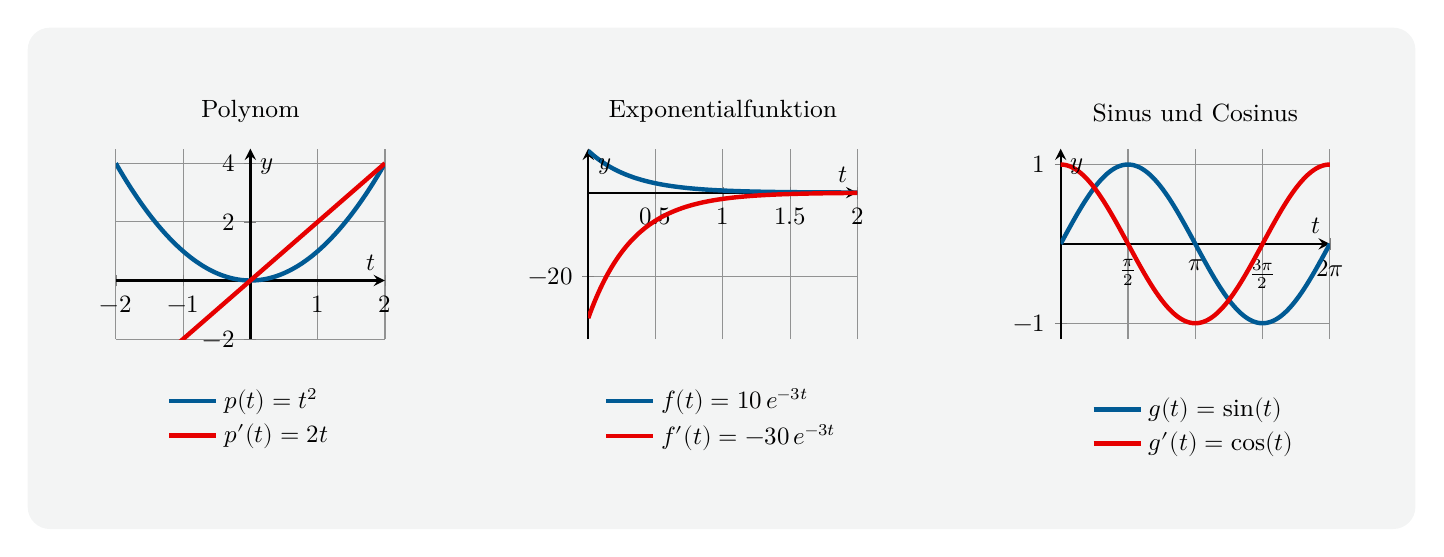
\begin{tikzpicture}[
    show background rectangle,
    background rectangle/.style={fill=my_lightgray, rounded corners=8pt},
    inner frame sep=0.8cm
]

% --- Panel 1: Polynom und Ableitung ------------------------------------
\begin{axis}[
    width = 5.0cm,
    height = 4.0cm,
    xshift = 0cm,
    axis lines = center,
    axis line style = {thick},
    xlabel = {$t$},
    ylabel = {$y$},
    xlabel style = {font=\small},
    ylabel style = {font=\small},
    grid = both,
    minor grid style = {draw=my_lightblue},
    major grid style = {draw=my_darkgray!60},
    ticklabel style = {font=\small},
    xmin = -2,
    xmax = 2,
    ymin = -2,
    ymax = 4.5,
    legend style = {
        font=\small,
        at={(0.5,-0.2)},
        anchor=north,
        draw=none,
        fill=none,
        /tikz/every even column/.style={column sep=0.5em}
    },
    legend cell align = left,
    title = {Polynom},
    title style = {font=\small},
    % axis equal hier bewusst weggelassen, damit der Verlauf gut erkennbar ist.
]

\addplot[
    draw = my_darkblue,
    ultra thick,
    samples = 300,
    domain = -2:2
]
{x^2};
\addlegendentry{$p(t) = t^2$};

\addplot[
    draw = my_red,
    ultra thick,
    samples = 300,
    domain = -2:2
]
{2*x};
\addlegendentry{$p'(t) = 2t$};

\end{axis}

% --- Panel 2: Exponentialfunktion und Ableitung ------------------------
\begin{axis}[
    width = 5.0cm,
    height = 4.0cm,
    xshift = 6.0cm,
    axis lines = center,
    axis line style = {thick},
    xlabel = {$t$},
    ylabel = {$y$},
    xlabel style = {font=\small},
    ylabel style = {font=\small},
    grid = both,
    minor grid style = {draw=my_lightblue},
    major grid style = {draw=my_darkgray!60},
    ticklabel style = {font=\small},
    xmin = 0,
    xmax = 2,
    ymin = -35,
    ymax = 10.5,
    legend style = {
        font=\small,
        at={(0.5,-0.2)},
        anchor=north,
        draw=none,
        fill=none,
        /tikz/every even column/.style={column sep=0.5em}
    },
    legend cell align = left,
    title = {Exponentialfunktion},
    title style = {font=\small},
    % axis equal hier bewusst weggelassen, damit der Abfall nach oben hin sichtbar bleibt.
]

\addplot[
    draw = my_darkblue,
    ultra thick,
    samples = 300,
    domain = 0:2
]
{10*exp(-3*x)};
\addlegendentry{$f(t) = 10\,e^{-3t}$};

\addplot[
    draw = my_red,
    ultra thick,
    samples = 300,
    domain = 0:2
]
{-30*exp(-3*x)};
\addlegendentry{$f'(t) = -30\,e^{-3t}$};

\end{axis}

% --- Panel 3: Sinus und Ableitung (Cosinus) ----------------------------
\begin{axis}[
    width = 5.0cm,
    height = 4.0cm,
    xshift = 12.0cm,
    axis lines = center,
    axis line style = {thick},
    xlabel = {$t$},
    ylabel = {$y$},
    xlabel style = {font=\small},
    ylabel style = {font=\small},
    grid = both,
    minor grid style = {draw=my_lightblue},
    major grid style = {draw=my_darkgray!60},
    ticklabel style = {font=\small},
    xmin = 0,
    xmax = 2*pi,
    ymin = -1.2,
    ymax = 1.2,
    xtick = {0, 1.5708, 3.1416, 4.7124, 6.2832},
    xticklabels = {$0$, $\frac{\pi}{2}$, $\pi$, $\frac{3\pi}{2}$, $2\pi$},
    legend style = {
        font=\small,
        at={(0.5,-0.25)},
        anchor=north,
        draw=none,
        fill=none,
        /tikz/every even column/.style={column sep=0.5em}
    },
    legend cell align = left,
    title = {Sinus und Cosinus},
    title style = {font=\small},
    % axis equal hier bewusst weggelassen, um beide Kurven in y-Richtung gut zu sehen.
]

\addplot[
    draw = my_darkblue,
    ultra thick,
    samples = 300,
    domain = 0:2*pi
]
{sin(deg(x))};
\addlegendentry{$g(t) = \sin(t)$};

\addplot[
    draw = my_red,
    ultra thick,
    samples = 300,
    domain = 0:2*pi
]
{cos(deg(x))};
\addlegendentry{$g'(t) = \cos(t)$};

\end{axis}

\end{tikzpicture}

\end{document}